\chapter{蒙特卡罗法}
\label{ch:monte_carlo}
随机算法有两个类别:拉斯维加斯(Las Vegas)算法和蒙特卡罗(Monte Carlo)算法(后简称蒙特卡罗法). 拉斯维加斯算法总是准确地返回正确的结果(或者失败). 这类算法需要随机数量的资源,通常是时间或者内存. 
而蒙特卡罗法返回有着随机错误率的结果. 错误率一般可以通过增加资源(如运行时间和内存)降低. 对任何固定的计算预算,蒙特卡罗法可以给出一个近似结果. \\

很多机器学习中的问题太过困难以至于我们无法期望得到准确的解. 这和准确的确定型算法和拉斯维加斯算法区分开来. 我们必须使用确定型近似算法或者蒙特卡罗近似. 




在 16.2.2 节,我们看到了很多概率模型(通常是无向图模型)是由一个没有正规化的概率分布 $\tilde{p}(\mathbf{x};\theta)$ 定义的. 我们必须通过除以一个配分函数 $Z(\pmb{\theta})$ 来正规化 $\tilde{p}$ 才能得到一个合法的概率分布:

\begin{equation}  \label{eq:pyth}
p(\mathbf{x};\pmb{\theta}) = \frac{1}{Z(\pmb{\theta})} \tilde{p}(\mathbf{x}; \pmb{\theta}).
\end{equation}

配分函数对连续型变量是积分,而对离散型变量是对所有状态的非正规化概率进行求和:

\begin{equation}  \label{eq:pyth}
\int \!\tilde{p}(\pmb{x})\, \mathrm{d}\pmb{x}
\end{equation}

或者

\begin{equation}  \label{eq:pyth}
\sum_{x} \tilde{p}(\pmb{x}).
\end{equation}

这个操作对很多有趣的模型都是难解的. 

如我们将在第 20 章中看到的,有些深度学习模型被设计成有可解的正规化常量,或者被设计成不需要包含计算 $p(\mathbf{x})$ 的. 然而,其他的模型需要直接面对难解的配分函数的挑战. 本章,我们会给出一些用来训练和评估那些有着难解配分函数的模型的技术. 

\section{对数似然梯度 log-likelihood gradient}
\label{sec:llg}

让通过最大似然估计在学习无向的模型中尤其困难的原因是配分函数依赖于参数. 对数似然函数关于参数的梯度包含一个配分函数的梯度项:

\begin{equation}  \label{eq:pyth}
\nabla_{\pmb{\theta}} \log p(\mathbf{x};\pmb{\theta}) = \nabla_{\pmb{\theta}} \log \tilde{p}(\mathbf{x};\pmb{\theta}) - \nabla_{\pmb{\theta}} \log Z(\pmb{\theta})
\end{equation}

这是一个著名的分解——将学习分成正负两个部分.\\

对大多数有趣的无向图模型,负部(negative phase)是困难的. 没有隐含变量或者隐含变量间的交互很少的模型通常会有可解的正部(positive phase) 典型的包含一个直接简单的正部而非常困难的负部的模型是 RBM,它的隐含单元在给定可见单元的时候是彼此是条件独立的. 而正部困难的例子是,隐含元之间的交互特别复杂,这个在第 19 章会讲述. 本章聚焦在负部的难解性上.\\

让我们仔细看看 $\log Z$ 的梯度:

\begin{equation}  \label{eq:pyth}
\frac{\partial}{\partial \pmb{\theta}} \log Z
\end{equation}
\begin{equation}  \label{eq:pyth}
=\frac{\frac{\partial}{\partial \pmb{\theta}} Z}{Z}
\end{equation}
\begin{equation}  \label{eq:pyth}
=\frac{\frac{\partial}{\partial \pmb{\theta}} \sum_{\mathbf{x}} \tilde{p}(\mathbf{x})}{Z}
\end{equation}
\begin{equation}  \label{eq:pyth}
=\frac{\sum_{\mathbf{x} \frac{\partial}{\partial \pmb{\theta}}} \tilde{p}(\mathbf{x})}{Z}
\end{equation}

对于那些对所有的 $\mathbf{x}$ 保证 $p(\mathbf{x}) > 0$ 的模型,我们可以为 $\tilde{p}(\mathbf{x})$ 替换 $\exp(\log \tilde{p}(\mathbf{x})$:
\begin{equation}  \label{eq:pyth}
\frac{\sum_{\mathbf{x}} \frac{\partial}{\partial \pmb{\theta}} \exp(\log \tilde{p}(\mathbf{x}))}{Z}
\end{equation}
\begin{equation}  \label{eq:pyth}
=\frac{\sum_{\mathbf{x}} \exp(\log\tilde{p}(\mathbf{x})) \frac{\partial}{\partial \pmb{\theta}} \tilde{p}(\mathbf{x})}{Z}
\end{equation}
\begin{equation}  \label{eq:pyth}
=\frac{\sum_{\mathbf{x}} \tilde{p}(\mathbf{x}) \frac{\partial}{\partial \pmb{\theta}} \tilde{p}(\mathbf{x})}{Z}
\end{equation}
\begin{equation}  \label{eq:pyth}
=\sum_{x}p(\mathbf{x}) \frac{\partial}{\partial \pmb{\theta}} \log \tilde{p}(\mathbf{x})
\end{equation}
\begin{equation}  \label{eq:pyth}
=\mathbf{E}_{x\sim p(\mathbf{x})} \frac{\partial}{\partial \pmb{\theta}} \tilde{p}(\mathbf{x}).
\end{equation}

这个推导对离散的 $\pmb{x}$ 进行求和,类似地也可以对连续的 $\pmb{x}$ 进行积分. 在连续版本的推到中,我们使用 Leibniz 法则在积分符号下进行微分,获得等式:
\begin{equation}  \label{eq:pyth}
\frac{\partial}{\partial \pmb{\theta}} \int \!\tilde{p}(\mathbf{x}) \, \mathrm{d}\pmb{x} = \int \!\frac{\partial}{\partial \pmb{\theta}} \tilde{p}(\pmb{x}) \,\mathrm{d}\pmb{x}.
\end{equation}

等式只有在 $\tilde{p}$ 和 $\frac{\partial}{\partial \pmb{\theta}} \tilde{p}(\mathbf{x})$ 满足某种规范化条件时可用. 用测度论的术语,条件是:
\begin{enumerate*}[label={\roman*)}]
\item $\tilde{p}$ 必须是一个对每个 $\pmb{\theta}$ 值的 $\pmb{x}$ 的 Lebesgue-可积函数;
\item $\frac{\partial}{\partial \pmb{\theta}} \tilde{p}(\mathbf{x})$ 必须对所有的 $\pmb{\theta}$ 和几乎所有的 $\pmb{x}$ 存在
\item 必须存在一个可积分函数 $R(\pmb{x})$ 控制住 $\frac{\partial}{\partial \pmb{\theta}} \tilde{p}(\mathbf{x})$(如对所有的 $\pmb{\theta}$ 和几乎所有的 $\pmb{x}$ 有 $|\frac{\partial}{\partial \pmb{\theta}}\tilde{p}(\mathbf{x})|\leq R(\pmb{x})$).
\end{enumerate*}

幸运的是,大多数机器学习模型满足这些条件.\\

这个等式
\begin{equation}  \label{eq:pyth15}
\nabla_{\pmb{\theta}} \log Z = \mathbb{E}_{\mathbf{x}\sim p(\mathbf{x})} \nabla_{\pmb{\theta}} \log \tilde{p}(\mathbf{x})
\end{equation}
是一系列 Monte Carlo 方法的基础,可以用来近似最大化那些有着难解的配分函数的模型的似然函数.\\

学习无向模型的 Monte Carlo 方法给出了一个直觉框架,我们可以利用这样的框架来思考正部和负部. 在正部中,我们对那些从数据抽取的 $\pmb{x}$ 增加 $\log \tilde{p}(\mathbf{x})$. 在负部中,我们通过减少从模型分布中个采样的 $\log \tilde{p}(\mathbf{x})$ 来降低配分函数.\\

在深度学习文献中,通常会用能量函数参数化 $\log \tilde{p}$(Eq. 16.7). 在这种情况下,我们可以将正部解释为降低训练样本的能量,而负部则是提升从模型中采样的样本的能量,如图 18.1 所示.

\section{随机最大似然和对比散度}

实现 \eqref{eq:pyth15} 的基本方式是每次需要计算梯度时从一个随机初始化状态的 Markov 链的集合中进行老化(burning). 在使用随机梯度下降算法进行学习时,这个 Markov 链必须每个梯度步都已经老化. 这个想法就是算法~\ref{alg:mcmc}
中的训练过程. 内循环中的 Markov 链老化的计算代价让这个过程在计算上不可行,但是这个过程本身是其他实效的近似算法的起点. 

% \begin{algorithm}[H]
%     设置 $\epsilon$,一个很小的正数作为步长.
%     设置 $\k$,Gibbs 步数,足够长满足老化条件. 在一个小的图像块(image patch)上训练 RBM 可能需要 $100$.


%   \caption{用来最大化对数似然函数的 MCMC 算法,使用梯度下降来处理难解的配分函数}
%   \label{alg:algorithm1}
% \end{algorithm}

\begin{algorithm}
\begin{algorithmic}
\caption{用来最大化对数似然函数的 MCMC 算法,使用梯度下降来处理难解的配分函数}
\label{alg:mcmc}
\STATE 设置 $\epsilon$,一个很小的正数作为步长.
\STATE 设置 $k$,Gibbs 步数,足够长满足老化条件. 在一个小的图像块(image patch)上训练 RBM 可能需要 $100$.
\WHILE{未收敛}
	\STATE 从训练集中采样 $m$ 个样本 $\{x^{(1)},\dots,x^{(m)}\}$ 的一个\gls{minibatch}.
	\STATE $\mathbf{g} \leftarrow \frac{1}{m}\,\sum_{i = 1}^{m} \nabla_{\pmb{\theta}} \log\tilde{p}(x^{(i)};\pmb{\theta})$.
	\STATE 将随机值为对应 $m$ 个样本 $\{\tilde{\mathbf{x}}^{(1)},\dots,\tilde{\mathbf{x}}^{(m)}\}$ 初始化(如,从一个均匀分布或者正态分布,或者也可能是有匹配于模型边缘分布的分布).
	\FOR{$i = 1$ to $k$}
	 	\FOR{$j = 1$ to $m$}
		\STATE $\tilde{\mathbf{x}}^{(j)} \leftarrow \mathrm{gibbs\_update}(\tilde{\mathbf{x}}^{(j)})$
		\ENDFOR
	\ENDFOR
	\STATE $\mathbf{g} \leftarrow \frac{1}{m}\,\sum_{i = 1}^{m} \nabla_{\pmb{\theta}} \log\tilde{p}(x^{(i)};\pmb{\theta})$.
	\STATE $\pmb{\theta} \leftarrow \pmb{\theta} + \epsilon \mathbf{g}$.
\ENDWHILE

\end{algorithmic}
\end{algorithm}

我们可以将最大似然 MCMC 方法看成是尝试达到两个力量的平衡,一个力量在数据出现时将模型分布上推,而另一个则在模型的样本出现时下推模型分布. 
图~\ref{fig:18.1}

% \begin{figure}
% \centering 
% 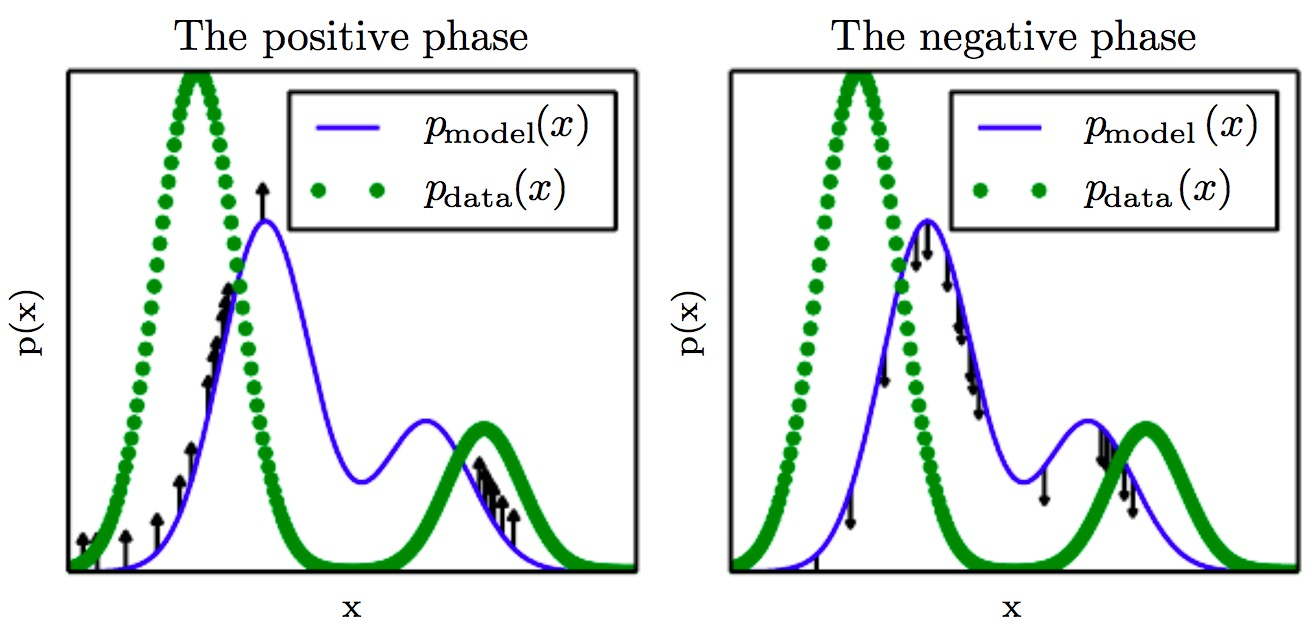
\includegraphics[width=1.0\textwidth]{figure18-1} 
% \caption{算法~\ref{alg:mcmc} 的正部和负部. 左图,在正部中,我们从数据分布中采样,上推他们的未规范化概率. 可能在数据中的点被更多地上推. 右图,在负部中,我们从模型的概率分布采样,下推他们的未规范化概率. 这样会抵制正部的倾向于在每个处都给未规范化概率加上一个大的常量. 当数据分布和模型分布等同时,正部和负部分别有同样的机会上推和下推. 这种情形出现时,就不再回产生梯度(期望形式),训练必须终止.}
% \label{fig:18.1} 
% \end{figure}

\begin{figure}[htp]
\centering 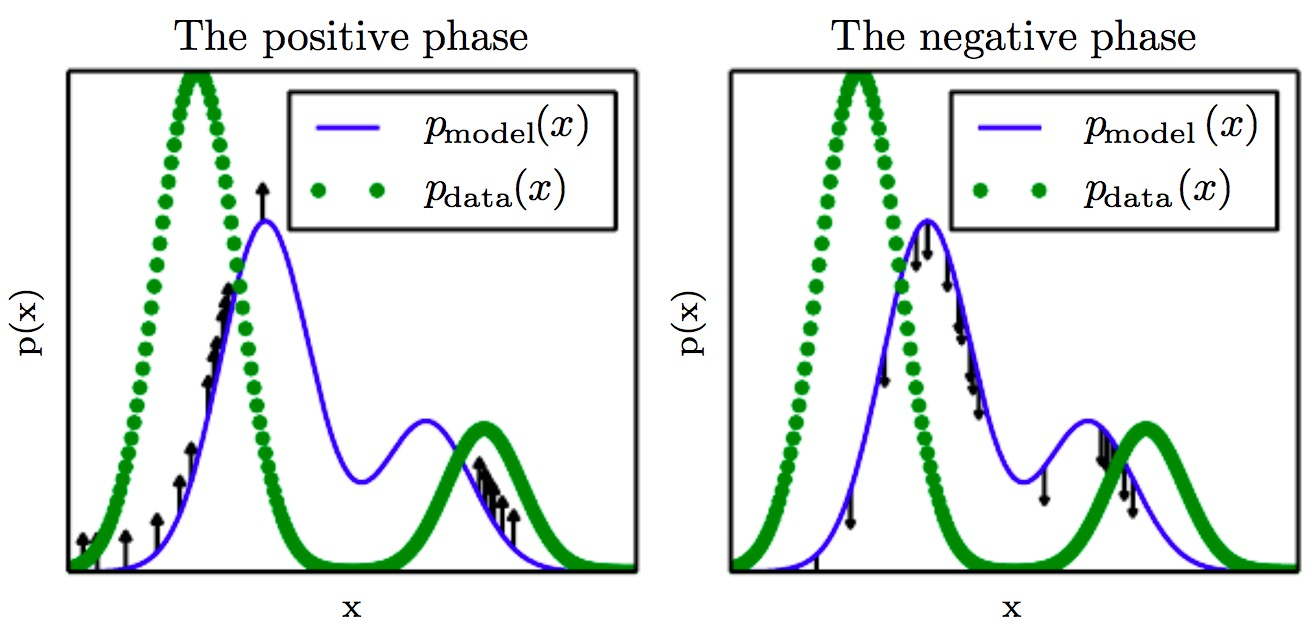
\includegraphics[width=1.0\textwidth]{figure18-1} 
\caption{算法~\ref{alg:mcmc} 的正部和负部. 左图,在正部中,我们从数据分布中采样,上推他们的未规范化概率. 可能在数据中的点被更多地上推. 右图,在负部中,我们从模型的概率分布采样,下推他们的未规范化概率. 这样会抵制正部的倾向于在每个处都给未规范化概率加上一个大的常量. 当数据分布和模型分布等同时,正部和负部分别有同样的机会上推和下推. 这种情形出现时,就不再回产生梯度(期望形式),训练必须终止.} 
\label{fig:18.1}
\end{figure}



